%%%%%%%%%%%%%%% LaTeX Compiler: XeLaTeX %%%%%%%%%%%%%%%

% License for LaTeX Configuration File

% This LaTeX configuration file is created by Lin, Xuanyu, HKUST, and is provided under the terms of the MIT License. You are free to use, copy, modify, merge, publish, distribute, sublicense, and/or sell copies of this configuration file, subject to the following conditions:

% 1. The above copyright notice and this license notice shall be included in all copies or substantial portions of the configuration file.

% 2. The configuration file is provided "as is", without warranty of any kind, express or implied, including but not limited to the warranties of merchantability, fitness for a particular purpose and noninfringement. In no event shall the authors or copyright holders be liable for any claim, damages or other liability, whether in an action of contract, tort or otherwise, arising from, out of or in connection with the configuration file or the use or other dealings in the configuration file.

% By using this configuration file, you agree to the terms and conditions of this license. If you do not agree to these terms and conditions, you must not use the configuration file.

\documentclass[10pt]{article}
% Text setting
% \usepackage{newtxtext}
\usepackage{setspace}
\usepackage[dvipsnames,svgnames]{xcolor}
\usepackage{comment}
% Chinese characters setup
\usepackage{fontspec}
\usepackage{xeCJK}
\setCJKmainfont{SimSun}
% Dealing with special characters
\usepackage[utf8]{inputenc}
% \usepackage[T1]{fontenc} % Conflict with fontspec & xeCJK
\usepackage{pifont}
% Mathematical formula typesetting
\usepackage{unicode-math}
\usepackage{amsmath}
\usepackage{amsfonts}
\usepackage{mathrsfs}
\setmathfont{Latin Modern Math}
% \usepackage{amssymb} % Contained in package unicode-math
% Jump (Math) \llbracket & \rrbracket
\usepackage{stmaryrd}
% Chemical formulas and equations
\usepackage[version=4]{mhchem}
% Graphics
\usepackage{graphicx}
\graphicspath{ {./images/} }
\usepackage[export]{adjustbox}
% Tables, enumeration
\usepackage{multirow}
\usepackage{caption}
\usepackage{subcaption}
\usepackage{enumitem}
% Adjust the position
\usepackage{float}
% Frames, reference
\usepackage{framed}
\usepackage[strict]{changepage}
\usepackage{hyperref}
\hypersetup{
	colorlinks=true,
	linkcolor=black,
	filecolor=magenta,      
	urlcolor=blue,
}
% Page & paragraph settings
\usepackage{fancyhdr}
\usepackage{geometry}
\geometry{left=1.5cm, right=1.5cm, top=2cm, bottom=2cm}
\usepackage{indentfirst}
\setlength{\parindent}{2em}
\setlength{\parskip}{0em}
% Algorithm & coding environment
\usepackage[ruled,vlined]{algorithm2e}
\usepackage[framemethod=TikZ]{mdframed}
\usepackage{listings}
\usepackage{wrapfig}
\usepackage{booktabs}
\usepackage{makecell}
% New command
\newcommand\course{COMP 3711}  
\newcommand\coursetitle{Design and Analysis of Algorithms}
\newcommand\semester{Fall 2023}
\renewcommand{\labelenumi}{\alph{enumi}}
\newcommand{\Z}{\mathbb Z}
\newcommand{\R}{\mathbb R}
\newcommand{\Q}{\mathbb Q}
\newcommand{\NN}{\mathbb N}
\newcommand{\dd}{\mathrm{d}}
\DeclareMathOperator{\Mod}{Mod}
\renewcommand\lstlistingname{Algorithm}
\renewcommand\lstlistlistingname{Algorithms}
\def\lstlistingautorefname{Alg.}

%%%%%%%%%%%%%%% Page Setup %%%%%%%%%%%%%%%

\pagestyle{fancy}
\headheight 35pt
\lhead{\course\ \coursetitle\ \semester}
\rhead{
\includegraphics[width=2.5cm]{logo-hkust.png}}
\lfoot{}
\pagenumbering{arabic}
\cfoot{}
\rfoot{\small\thepage}
\headsep 1.2em

%%%%%%%%%%%%%%% Boxframe Setup %%%%%%%%%%%%%%%

\definecolor{blueshade}{rgb}{0.95,0.95,1} % Horizontal Line: DarkBlue
\definecolor{greenshade}{rgb}{0.90,0.99,0.91} % Horizontal Line: Green
\definecolor{redshade}{rgb}{1.00,0.90,0.90}% Horizontal Line: LightCoral
\definecolor{brownshade}{rgb}{0.99,0.97,0.93} % Horizontal Line: BurlyWood

\newenvironment{formal}[2]{%
	\def\FrameCommand{%
		\hspace{1pt}%
		{\color{#1}\vrule width 2pt}%
		{\color{#2}\vrule width 4pt}%
		\colorbox{#2}%
	}%
	\MakeFramed{\advance\hsize-\width\FrameRestore}%
	\noindent\hspace{-4.55pt}% Disable indenting first paragraph
	\begin{adjustwidth}{}{7pt}%
		\vspace{2pt}\vspace{2pt}%
	}
	{%
		\vspace{2pt}\end{adjustwidth}\endMakeFramed%
}

%%%%%%%%%%%%%%% Problem Environment Setup %%%%%%%%%%%%%%%

\mdfdefinestyle{problemstyle}{
	linecolor=black,linewidth=1pt,
	frametitlerule=true,
	frametitlebackgroundcolor=gray!20,
	roundcorner=10pt,
	innertopmargin=\topskip,
	frametitlealignment=\hspace{0em},
}

\mdfsetup{skipabove=\topskip,skipbelow=\topskip}
\mdtheorem[style=problemstyle]{Problem}{Problem}
\newenvironment{Solution}{\textbf{Solution.}}

%%%%%%%%%%%%%%% Coding Environment S6etup %%%%%%%%%%%%%%%

\lstset{
	basicstyle=\tt,
	% Line number
	numbers=left,
	rulesepcolor=\color{red!20!green!20!blue!20},
	escapeinside=``,
	xleftmargin=2em,xrightmargin=2em, aboveskip=1em,
	% Background frame
	framexleftmargin=1.5mm,
	frame=shadowbox,
	% Background color
	backgroundcolor=\color[RGB]{252,236,227},
	% Style
	keywordstyle=\color{blue}\bfseries,
	identifierstyle=\bf,
	numberstyle=\color[RGB]{0,192,192},
	commentstyle=\it\color[RGB]{0,153,51},
	stringstyle=\rmfamily\slshape\color[RGB]{128,0,0},
	% Show space
	showstringspaces=false
}

%%%%%%%%%%%%%%% Document Begins %%%%%%%%%%%%%%%

\begin{document}
	
%%%%%%%%%%%%%%% Title Page %%%%%%%%%%%%%%%

\begin{titlepage}
	\begin{center}
		\vspace*{3cm}
		
		\Huge
		\hrulefill
		\vspace{1cm}
		
		\huge
		\textbf{COMP 3711 Course Notes\\}
		\vspace{1cm}
		\textbf{Design and Analysis of Algorithms}
		\vspace{1cm}
		
		\hrulefill
		
		\vspace{1.5cm}
		\Large

		\textbf{LIN, Xuanyu}
		
		\vfill
		
		$\mathscr{ALGORITHMS}$
		
		\vspace{1cm}
		
		\course \ Design and Analysis of Algorithms
		
		\vspace{1cm}
		
		
\includegraphics[width=0.4\textwidth]{logo-hkust.png}
		\\
		
		\Large
		
		\today
		
	\end{center}
\end{titlepage}

%%%%%%%%%%%%%%% Article Begins %%%%%%%%%%%%%%%

\begin{comment}

\begin{abstract}
	Abstract Abstract Abstract Abstract Abstract Abstract Abstract Abstract Abstract Abstract Abstract Abstract Abstract Abstract Abstract Abstract Abstract Abstract Abstract Abstract Abstract Abstract Abstract Abstract Abstract Abstract Abstract Abstract Abstract Abstract Abstract Abstract Abstract
\end{abstract}

\tableofcontents

\begin{center}
	\section*{\LARGE Title}
\end{center}

\section{Section 1}

This is a link to \href{https://www.google.com}{Google}.

$$
\vec{\nabla} \cdot \vec{E}=\frac{1}{\epsilon_{0}} \cdot \rho
$$

\begin{formal}{DarkBlue}{blueshade}
	\textbf{Theorem 1.1} 这是一段中文。\hyperref[ref1]{[1]}
	
	$$
	\vec{\nabla} \cdot \vec{E}=\frac{1}{\epsilon_{0}} \cdot \rho
	$$
	
	\noindent This is an English sentence.
\end{formal}


\begin{center}
	\begin{tabular}{|c|c|c|}
		\hline
		\multirow{2}{*}{A} & B & C \\
		\cline{2-3}
		& D & E \\
		\hline
	\end{tabular}
\end{center}

\begin{algorithm}
	\SetAlgoLined
	\KwIn{$a, b$}
	\KwOut{$c$}
	$c = a + b$\;
	\Return{$c$}\;
	\caption{Addition}
\end{algorithm}

\begin{Problem}[Title]
	
	\lstset{language=Python}
	\begin{lstlisting}[tabsize=4]
print("Hello World!")
	\end{lstlisting}

\end{Problem}

\begin{Solution}
	
	Text
	
\end{Solution}

\section{References}

\label{ref1}

[1] Google \href{https://www.google.com}{https://www.google.com}

\end{comment}

\tableofcontents

\newpage

\section{Asymptotic Notation}

\begin{formal}{DarkBlue}{blueshade}
	
	\noindent \textbf{Upper Bounds} $T(n) = O(f(n))$
	
	if exist constants $c > 0$ and $n_0 \geq 0$ such that for all $n \geq n_0$, $T(n) \leq c \cdot f(n)$.
	
	\noindent \textbf{Lower Bounds} $T(n) = \Omega(f(n))$
	
	if exist constants $c > 0$ and $n_0 \geq 0$ such that for all $n \geq n_0$, $T(n) \geq c \cdot f(n)$.
	
	\noindent \textbf{Tight Bounds} $T(n) = \Theta(f(n))$
	
	if $T(n) = O(f(n))$ and $T(n) = \Omega(f(n))$.
	
	\noindent \textbf{Note:} Here "=" means "is", not equal.
	
\end{formal}

\section{Introduction - The Sorting Problem}

\subsection{Selection Sort}

\begin{algorithm}
	\SetAlgoLined
	\KwIn{An array $A[1 ... n]$ of elements}
	\KwOut{Array $A[1 ... n]$ of elements in sorted order (asending)}
	\For{$i \gets 1$ to $n-1$}{
		\For{$j \gets i+1$ to $n$}{
			\If{$A[i]>A[j]$}{
				swap $A[i]$ and $A[j]$
			}
		}
	}
	\caption{Selection Sort}
\end{algorithm}

Running Time: $\frac{n(n-1)}{2}$

Best-Case = Worst-Case: $T(n) = \Theta(\frac{n(n-1)}{2}) = \Theta(n^2)$

\subsection{Insertion Sort}

\begin{algorithm}
	\SetAlgoLined
	\KwIn{An array $A[1 ... n]$ of elements}
	\KwOut{Array $A[1 ... n]$ of elements in sorted order (asending)}
	\For{$i \gets 2$ to $n$}{
		$j \gets i-1$
		\While{$j \geq 1$ and $A[j] > A[j+1]$}{
			swap $A[j]$ and $A[j+1]$
		}
		$j \gets j-1$
	}
	\caption{Insertion Sort}
\end{algorithm}

Running Time: Depends on the input array, ranges between $(n-1)$ and $\frac{n(n-1)}{2}$

Best-Case: $T(n) = n-1 = \Theta(n)$ (Useless)

Worst-Case: $T(n) = \Theta(\frac{n(n-1)}{2}) = \Theta(n^2)$ (Commonly-Used)

Average-Case: $T(n) = \Theta(\sum_{i=2}^n \frac{i-1}{2}) = \Theta(\frac{n(n-1)}{4}) = \Theta(n^2)$ (Sometimes Used)

\subsection{Wild-Guess Sort}

\begin{algorithm}
	\SetAlgoLined
	\KwIn{An array $A[1 ... n]$ of elements}
	\KwOut{Array $A[1 ... n]$ of elements in sorted order (asending)}
	$\pi \gets [4,7,1,3,8,11,5,...]$\ \ Create random permutation
	Check if $A[\pi[i]] \leq A[\pi[i+1]]$ for all $i = 1,2,...,n-1$
	If yes, output A according to $\pi$ and terminate
	else $Insertion-Sort(A)$
	\caption{Wild-Guess Sort}
\end{algorithm}

Running Time: Depends on the random generation, could be faster than the insertion sort.

\subsection{Worst-Case Analysis}

The algorithm’s worst case running time is $O(f(n)) \implies $ On all inputs of (large) size $n$, the running time of the algorithm is $\leq c \cdot f(n)$.

The algorithm’s worst case running time is $\Omega (f(n)) \implies $ There exists at least one input of (large) size $n$ for which the running time of the algorithm is  $\geq c \cdot f(n)$.

Thus, Insertion sort runs in $\Theta (n^2)$ time.

\begin{formal}{DarkBlue}{blueshade}
	
	\textbf{Notice}
	
	Selection sort, insertion sort, and wild-guess sort all have worst-case running time $\Theta (n^2)$. How to distinguish between them?
	
	$\bullet$ Closer examination of hidden constants
	
	$\bullet$ Careful analysis of typical expected inputs
	
	$\bullet$ Other factors such as cache efficiency, parallelization are important
	
	$\bullet$ Empirical comparison
	
\end{formal}

\begin{formal}{DarkGreen}{greenshade}

	\textbf{Stirling's Formula}
	
	Prove that $\log (n!) = \Theta (n \log n)$
	
	First $\log (n!) = O (n \log n)$ since:
	
	$$
	\log (n!) = \sum_{i=1}^n \log i \leq n \times \log n = O (n \log n)
	$$

	Second $\log (n!) = \Omega (n \log n)$ since:
	
	$$
	\log (n!) = \sum_{i=1}^n \log i \geq \sum_{i=n/2}^n \log i \geq n/2 \times \log n/2 = n/2 (\log n - \log 2) = \Omega (n \log n)
	$$
	
	Thus, $\log (n!) = \Theta (n \log n)$

\end{formal}

\newpage

\section{Divide \& Conquer}

\textbf{Main idea of D \& C:} Solve a problem of size $n$ by breaking it into one or more smaller problems of size less than $n$. Solve the smaller problems recursively and combine their solutions, to solve the large problem.


\subsection{Binary Search}

\begin{formal}{Brown}{brownshade}
	
	\textbf{Example: Binary Search}
	
	\textbf{Input:} A sorted array $A[1,...,n]$, and an element $x$
	
	\textbf{Output:} Return the position of $x$, if it is in $A$; otherwise output nil
	
	\textbf{Idea of the binary search:} Set $q \gets$ middle of the array. If $x = A[q]$, return $q$. If $x < A[q]$, search $A[1,...,q-1]$, else search $A[q+1,...,n]$.
	
\end{formal}

\begin{algorithm}
	\SetAlgoLined
	\KwIn{Array $A[1 ... n]$ of elements in sorted order}
	\SetKwFunction{BinarySearch}{BinarySearch}
	\BinarySearch{$A[], p, r, x$}($p, r$ being the left \& right iteration, $x$ being the element being searched){
		
		\If{$p > r$}{
			\Return{nil}
		}
		$q \gets [(p+r)/2]$
		
		\If{$x = A[q]$}{
			\Return{$q$}
		}
		\If{$x < A[q]$}{
			\BinarySearch{$A[], p, q-1, x$}
		}
		\Else{
			\BinarySearch{$A[], q+1, r, x$}
		}
	}
	\caption{Binary Search}
\end{algorithm}

Recurrence of the algorithm, supposing $T(n)$ being the number of the comparisons needed for $n$ elements:

\noindent $T(n) = T(\frac{n}{2}) + 2$ if $n > 1$, with $T(1) = 2$.

$\implies T(n) = 2\log_2 n + 2 \implies O(\log n)$ algorithm

\begin{formal}{Brown}{brownshade}
	
	\textbf{Example: Binary Search in Rotated Array}
	
	Suppose you are given a sorted array $A$ of $n$ distinct numbers that 
	has been rotated $k$ steps, for some unknown integer $k$ between 1 and $n-1$. That is, $A[1 ... k]$ is sorted in increasing order, and $A[k+1 ... n]$ is also sorted in increasing order, and $A[n] < A[1]$.
	
	Design an $O(\log n)$-time algorithm that for any given x, 
	finds x in the rotated sorted array, or reports that it does not 
	exist.
	
	\noindent \textbf{Algorithm:}
	
	First conduct a $O(\log n)$ algorithm to find the value of $k$, then search for the target value in either the first part or the second part.
	
	$Find-x(A, x)$
	
	$k \leftarrow Find-k(A, 1, n)$ (First find $k$)
	
	$if\ x \geq A[1]\ then\ return\ BinarySearch(A, 1, k, x)$
	
	$Else\ return\ BinarySearch(A, k+1, n, x)$
	
\end{formal}

\newpage

\begin{formal}{Brown}{brownshade}
	
	\textbf{Example: Finding the last 0}
	
	You are given an array $A[1 ... n]$ that contains a sequence of 0 
	followed by a sequence of 1 (e.g., 0001111111). $A$ contains $k$ 0(s) ($k>0$ and $k<<n$) and at least one 1.
	
	Design an $O(\log k)$-time algorithm that finds the position $k$ of the last 0.

	\noindent \textbf{Algorithm:}
	
	$i\leftarrow1$
	
	$while\ A[i]=0$
	
	\quad \quad $i\leftarrow2i$
	
	$find-k(A[i/2 ... i])$

\end{formal}

\subsection{Merge Sort}

\textbf{Principle of the Merge Sort:}

$\bullet$ Divide array into two halves.

$\bullet$ Recursively sort each half.

$\bullet$ Merge two halves to make sorted whole.

\begin{algorithm}
	\SetAlgoLined
	\SetKwFunction{MergeSort}{MergeSort}
	\SetKwFunction{Merge}{Merge}
	\MergeSort{$A, p, r$}($p, r$ being the left \& right side of the array to be sorted){
		
		\If{$p = r$}{
			\Return
		}
		$q \gets [(p+r)/2]$
		
		\MergeSort{$A, p, q$}
		
		\MergeSort{$A, q+1, r$}
		
		\Merge{$A, p, q, r$}
		
		\underline{First Call:} \MergeSort{$A, 1, n$}
	}
	\caption{Merge Sort}
\end{algorithm}

\begin{algorithm}
	\SetAlgoLined
	\KwIn{Two Arrays $L\gets A[p ... q]$ and $R\gets A[q+1 ... r]$ of elements in sorted order}
	\SetKwFunction{Merge}{Merge}
	\Merge{$A, p, q, r$}{
		
		Append $\infty$ at the end of $L$ and $R$
		
		$i\gets 1,\ j\gets 1$
		
		\For{$k \gets p$ to $r$}{
		
			\If{$L[i] \leq R[j]$}{
				
				$A[k] \gets L[i]$
				
				$i \gets i + 1$

			}
		
			\Else{
			
				$A[k] \gets R[j]$
				
				$j \gets j + 1$
		
			}
			
		}

	}
	\caption{Merge}
\end{algorithm}

Let $T(n)$ be the running time of the algorithm on an array of size $n$.

\noindent \textbf{Merge Sort Recurrence:}
$$
T(n) \leq T(\lfloor n/2 \rfloor) + T(\lceil n/2 \rceil) + O(n), \quad n>1, \quad T(1) = O(1)
$$
\textbf{Simplification:}
$$
\implies T(n) = 2T(n/2) + n, \quad n>1, \quad T(1) = 1
$$
\textbf{Result:}
$$
T(n) = n\log_2 n + n = O(n\log n)
$$

\newpage

\subsection{Inversion Counting}

\textbf{Definition of the Inversion Numbers:} Given array $A[1 ... n]$, two elements $A[i]$ and $A[j]$ are inverted if $i < j$ but $A[i] > A[j]$. The inversion number of $A$ is the number of inverted pairs.

\begin{formal}{DarkBlue}{blueshade}
	
	\textbf{Theorem:}

	The number of swaps used by Insertion Sort = Inversion Number (Proved by induction on the size of the array)
	
	\noindent \textbf{Algorithm to Compute Inversion Number:}
	
	Algorithm 1: Check all $\Theta(n^2)$ pairs.
	
	Algorithm 2: Run Insertion Sort and count the number of swaps – Also $\Theta(n^2)$ time.
	
	Algorithm 3: Divide and Conquer
	
\end{formal}

\subsubsection{Counting Inversions: Divide-and-Conquer}

\textbf{Principle of the Algorithm:}

$\bullet$ Divide: divide array into two halves

$\bullet$ Conquer: recursively count inversions in each half

$\bullet$ Conbine: count inversions where $a_i$ and $a_j$ are in different halves, and return sum of three quantities

Inversion counting during the combine step is very similar to the Merge Algorithm (Algorithm 6), by counting the sum of each inversion number of the right array (indicated by $I[j]$) comparing to the left array.

\begin{algorithm}
	\SetAlgoLined
	\KwIn{Two Arrays $L\gets A[p ... q]$ and $R\gets A[q+1 ... r]$ of elements in sorted order}
	\SetKwFunction{Count}{Count}
	\Count{$A, p, q, r$}{
		
		$i\gets 1,\ j\gets 1,\ c\gets 0$
		
		\While{$(i \leq q-p+1) \&\& (j \leq r-q)$}{
			
			\If{$L[i] \leq R[j]$}{
				
				$i \gets i+1$
				
			}
			
			\Else{
				
				$I[j] = q-p-i+2$
				
				$c \gets c+I[j]$
				
				$j \gets j+1$
				
			}
			
		}
		
	}
	\caption{Inversion Count during Combination}
\end{algorithm}

The time-complexity of the algorithm is $\Theta(n\log n)$, same as the Merge Sort.

\subsubsection{Implementation of the Algorithm}

\begin{algorithm}
	\SetAlgoLined
	\SetKwFunction{Sort}{Sort-and-Count}
	\SetKwFunction{Merge}{Merge-and-Count}
	\Sort{$A, p, r$}{
		
		\If{$p = r$}{
			\Return{0}
		}
		$q \gets \lfloor(p+r)/2\rfloor$
		
		$c_1 \gets$ \Sort{$A, p, q$}
		
		$c_2 \gets$ \Sort{$A, q+1, r$}
		
		$c_3 \gets$ \Merge{$A, p, q, r$}
		
		\Return{$c_1 + c_2 + c_3$}
		
		\underline{First Call:} \Sort{$A, 1, n$}
	}
	\caption{Main Algorithm}
\end{algorithm}

\begin{algorithm}
	\SetAlgoLined
	\KwIn{Two Arrays $L\gets A[p ... q]$ and $R\gets A[q+1 ... r]$ of elements in sorted order}
	\SetKwFunction{Merge}{Merge-and-Count}
	\Merge{$A, p, q, r$}{
		
		Append $\infty$ at the end of $L$ and $R$
		
		$i\gets 1,\ j\gets 1, c\gets 0$
		
		\For{$k \gets p$ to $r$}{
			
			\If{$L[i] \leq R[j]$}{
				
				$A[k] \gets L[i]$
				
				$i \gets i + 1$
				
			}
			
			\Else{
				
				$A[k] \gets R[j]$
				
				$j \gets j + 1$
				
				$c \gets c+q-p-i+2$
				
			}
			
		}
	
		\Return{$c$}
		
	}
	\caption{Merge-and-Count}
\end{algorithm}

\subsection{Basic Summary of D\&C: Problem Size \& Number of Problems}

\textbf{Observations of D\&C in Logarithmic Patterns:}

$\bullet$ Break up problem of size $n$ into $p$ parts of size $n/q$.

$\bullet$ Solve parts recursively and combine solutions into overall solution.

$\bullet$ At level $i$, we break $i$ times and we have $p^i$ problems of size $n/q^i$.

$\bullet$ When we cannot break up any more, usually when the problem size 
becomes 1. Usually $i \approx \log_q n$.

\begin{formal}{DarkGreen}{greenshade}

The number of problems at (bottom) level $\log_q n$ is $p^i = p^{\log_q n} = n^{\log_q p}$.

\end{formal}

\vspace{1em}

\textbf{Observations of D\&C in Non-Logarithmic Patterns:}

$\bullet$ Break up problem of size $n$ into $p(\leq 2)$ parts of size $n-q$. (e.g. $q=1$ for Hanoi Problem)

$\bullet$ Assume that $q=1$

$\bullet$ At level i, we break $i$ times and we have $p^i$ problems of size $n-i$.

$\bullet$ If we stop when the problem size becomes 1, then $n-i=1 \implies i=n-1$.

\begin{formal}{DarkGreen}{greenshade}

The number of problems at (bottom) level $n-1$ is: $p^i = p^{n-1}$.

\end{formal}

\subsection{Maximum Contiguous Subarray}

\begin{formal}{Brown}{brownshade}
	
	\textbf{Example: The Maximum Subarray Problem}
	
	\textbf{Input:} An array of numbers $A[1,...,n]$, both positive and negative
	
	\textbf{Output:} Find the maximum $V(i, j)$, where $V(i, j) = \sum_{k=i}^j A[k]$
	
\noindent \textbf{Brute-Force Algorithm}

\textbf{Idea:} Calculate the value of $V(i, j)$ for each pair $i\leq j$ and return the maximum value.

Requires three nested for-loop, time complexity: $\Theta(n^3)$.

\noindent \textbf{A Data-Reuse Algorithm}

\textbf{Idea:} $V(i, j) = V(i, j-1) + A[j]$

Requires two nested for-loop, time complexity: $\Theta(n^2)$.

\end{formal}

\newpage

\subsubsection{A D\&C Algorithm}

\textbf{Idea:} Cut the array into two halves, all subarrays can be classified into three cases: entirely in the first/second half, or crosses the cut.

\textbf{Compare with the merge sort:} Whole algorithm will run in $\Theta(n\log n)$ time if the cross-cut can be solved in $O(n)$ time.

\begin{algorithm}
	\SetAlgoLined
	\SetKwFunction{MaxSubArray}{MaxSubArray}
	\MaxSubArray{$A, p, r$}{
		
		\If{$p = r$}{
			\Return{$A[p]$}
		}
		$q \gets \lfloor(p+r)/2\rfloor$
		
		$M_1 \gets$ \MaxSubArray{$A, p, q$}
		
		$M_2 \gets$ \MaxSubArray{$A, q+1, r$}
		
		$L_m, R_m \gets -\infty$
		
		$V \gets 0$
		
		\For{$i \gets q$ to $p$}{
		
			$V \gets V+A[i]$
			
			\If{$V>L_m$}{
			
				$L_m \gets V$
			
			}
		
		}
	
		$V \gets 0$
		
		\For{$i \gets q+1$ to $r$}{
			
			$V \gets V+A[i]$
			
			\If{$V>R_m$}{
				
				$R_m \gets V$
				
			}
			
		}
		
		\Return{$\max(M_1, M_2, L_m+R_m)$}
		
		\underline{First Call:} \MaxSubArray{$A, 1, n$}
	}
	\caption{Maximum Subarray}
\end{algorithm}

\textbf{Recurrence:} $T(n) = 2T(n/2)+n \implies T(n) = \Theta(n\log n)$

\subsubsection{Kadane's Algorithm}

\textbf{Idea:} Based on the principles of \textbf{Dynamic Programming}. Let $V[i]$ be the (local) maximum sub-array that ends at $A[i]$, then we let:

$\bullet V[1] = A[1]$

$\bullet V[i] = \max(A[i], A[i] + V[i-1])$

The maximum of $V[i]$, namely $V_{max}$ is the maximum continuous subarray found so far.

\begin{algorithm}
	\SetAlgoLined
	
	$V_{max} \gets -\infty; V \gets 0; \text{start} \gets 1; \text{end} \gets 1; \text{temp} \gets 1$ (Note: start \& end specify the maximum sub-array)
		
	\For{$i\gets 1$ to $n$}{
	
	$V\gets V+A[i]$
	
	\If(// Implies $V[i-1]$ is negative, restart from the current position){$V < A[i]$}{
		
		$V\gets A[i]; \text{temp}\gets i$
		
		}

	\If(// Found a max sum, update start and end){$V > V+{max}$}{
	
		$V_{max}\gets V; \text{start}\gets \text{temp}; \text{end}\gets i$

		}

	}
	
	\caption{Kadane's Algorithm}
\end{algorithm}

\textbf{Time Complexity:} $\Theta(n)$

\begin{formal}{Brown}{brownshade}
	
	\textbf{Example: Maximizing Stock Profits}
	
	You are presented with an array $p[1\dots n]$ where $p[i]$ is the price of the stock on day $i$.
	
	Design an divide-and-conquer algorithm that finds a strategy to make as much money as possible, i.e., it finds a pair $i, j$ with $1\leq i\leq j\leq n$ such that $p[j]-p[i]$ is maximized over all possible such pairs. Note that you are only allowed to buy the stock once and then sell it later.

\vspace*{1em}

\noindent \textbf{Idea 1: Divide and Conquer}

$\bullet$ Cut the array into two halves.

$\bullet$ All $i, j$ solutions can be classified into three cases: both $i, j$ are entirely in the first(second) half, or $i$ is in the left half while $j$ is in the right half.

$\bullet$ Maximizing a Case 3 result $p[j]-p[i]$ means finding the smallest value in the first half and the largest in the second half.

\textbf{Time Complexity:} $T(n) = 2T(n/2) + n \implies T(n) = \Theta(n\log n)$

\vspace*{1em}

\noindent \textbf{Idea 2: Kadane's Algorithm}

$\bullet$ Create a \textbf{Profit} array with $Profit[i]=Price[i+1]-Price[i]$.

$\bullet$ Perform the Kadane's Algorithm.

\textbf{Time Complexity:} $O(n)$

\end{formal}

\subsection{Integer Multiplication}

\subsubsection{A Simple D\&C Algorithm for Integer Multiplication}

\textbf{Goal:} Given two $n$-bit binary integers $a$ and $b$, compute: $a\cdot b$.

\textbf{Idea:} Multiplication by $2^k$ can be done in one time unit by a left shift of $k$ bits.

$\bullet$ Rewrite the two numbers as $a = 2^{n/2} a_1 + a_0$, $b = 2^{n/2} b_1 + b_0$.

$\bullet$ The product becomes: $a\cdot b = (2^{n/2} a_1 + a_0)(2^{n/2} b_1 + b_0) = 2^n a_1 b_1 + 2^{n/2} (a_1 b_0 + a_0 b_1) + a_0 b_0$

$\bullet$ The new computation requires 4 products of integers, each with $n/2$ bits.

$\bullet$ Apply D\&C by splitting a problem of size $n$, to 4 problems of size $n/2$.

\begin{algorithm}
	\SetAlgoLined
	\SetKwFunction{Multiply}{Multiply}
	\Multiply{$A, B$}{
		
		$n\gets$ size of $A$
		
		\If{$n = 1$}{\Return{$A[1]\cdot B[1]$}}
		
		$mid \gets \lfloor n/2 \rfloor$
		
		$U \gets$ \Multiply($A[mid+1..n], B[mid+1..n]$) // $a_1b_1$
		
		$V \gets$ \Multiply($A[mid+1..n], B[1..mid]$) // $a_1b_0$
		
		$W \gets$ \Multiply($A[1..mid], B[mid+1..n]$) // $a_0b_1$
		
		$Z \gets$ \Multiply($A[1..mid], B[1..mid]$) // $a_0b_0$
		
		$M[1..2n]\gets 0$
		
		$M[1..n]\gets Z$ // $a_0b_0$
		
		$M[mid+1..]\gets M[mid+1..] \oplus V \oplus W$ // $+[(a_1b_0+a_0b_1)\ll\text{(left shift) } n/2]$
		
		$M[2mid+1..]\gets M[2mid+1..] \oplus U$ // $+[a_1b_1\ll n]$
		
		\Return{$M$}
		
	}
	\caption{Binary Multiplication}
\end{algorithm}

\textbf{Time Complexity:} $T(n) = 4T(n/2) + n\implies T(n) = \Theta(n^2)$

\newpage

\subsubsection{Karatsuba Multiplication}

\textbf{Goal:} Given two $n$-bit binary integers $a$ and $b$, compute: $a\cdot b$.

\textbf{Idea:}

$\bullet$ We've seen that $ab = a_1b_1 2^n + (a_1b_0+a_0b_1) 2^{n/2} + a_0b_0$, so we only need the result of $a_1b_0+a_0b_1$.

$\bullet$ Note that $a_1b_0+a_0b_1 = (a_1+a_0)(b_1+b_0) - a_1b_1 - a_0b_0$, thus only requires performing 3 multiplications of size $n/2$.

\begin{algorithm}
	\SetAlgoLined
	\SetKwFunction{Multiply}{Multiply}
	\Multiply{$A, B$}{
		
		$n\gets$ size of $A$
		
		\If{$n = 1$}{\Return{$A[1]\cdot B[1]$}}
		
		$mid \gets \lfloor n/2 \rfloor$
		
		$U \gets$ \Multiply($A[mid+1..n], B[mid+1..n]$) // $a_1b_1$
		
		$Z \gets$ \Multiply($A[1..mid], B[1..mid]$) // $a_0b_0$
		
		$A'\gets A[mid+1..n] \oplus A[1..mid]$ // $a_1+a_0$
		
		$B'\gets B[mid+1..n] \oplus B[1..mid]$ // $b_1+b_0$
		
		$Y \gets$ \Multiply($A', B'$) // $(a_1+a_0)(b_!+b_0)$
		
		$M[1..2n]\gets 0$
		
		$M[1..n]\gets Z$ // $a_0b_0$
		
		$M[mid+1..]\gets M[mid+1..] \oplus Y \ominus U \ominus Z$ // $+[(a_1b_0+a_0b_1)\ll\text{(left shift) } n/2]$
		
		$M[2mid+1..]\gets M[2mid+1..] \oplus U$ // $+[a_1b_1\ll n]$
		
		\Return{$M$}
		
	}
	\caption{Binary Multiplication (Karatsuba's Multiplication Algorithm)}
\end{algorithm}

\textbf{Time Complexity:} $T(n) = 3T(n/2) + n\implies T(n) = \Theta(n^{\log_2 3}) = \Theta(n^{1.585\cdots})$

For recent research, see: \href{https://annals.math.princeton.edu/2021/193-2/p04}{Integer Multiplication in $O(n\log n)$ Time (David Harvey \& Joris van der Hoeven, 2021)}

\subsection{Matrix Multiplication}

$$
\left[
\begin{matrix}
	c_{11} & c_{12} & \cdots & c_{1n}\\
	c_{21} & c_{22} & \cdots & c_{2n}\\
	\cdots & \cdots & \cdots & \cdots\\
	c_{n1} & c_{n2} & \cdots & c_{nn}
\end{matrix}
\right]
=
\left[
\begin{matrix}
	a_{11} & a_{12} & \cdots & a_{1n}\\
	a_{21} & a_{22} & \cdots & a_{2n}\\
	\cdots & \cdots & \cdots & \cdots\\
	a_{n1} & a_{n2} & \cdots & a_{nn}
\end{matrix}
\right]
\left[
\begin{matrix}
	b_{11} & b_{12} & \cdots & b_{1n}\\
	b_{21} & b_{22} & \cdots & b_{2n}\\
	\cdots & \cdots & \cdots & \cdots\\
	b_{n1} & b_{n2} & \cdots & b_{nn}
\end{matrix}
\right]\quad
c_{ij} = \sum_{k=1}^n a_{ik} b_{kj}
$$

\textbf{Brute Force Method:} $\Theta (n^3)$ time.

\subsubsection{A D\&C Solution to Matrix Multiplication}

$$
\left[
\begin{matrix}
	C_{11} & C_{12}\\
	C_{21} & C_{22}
\end{matrix}
\right]
=
\left[
\begin{matrix}
	B_{11} & B_{12}\\
	B_{21} & B_{22}
\end{matrix}
\right]
\left[
\begin{matrix}
	A_{11} & A_{12}\\
	A_{21} & A_{22}
\end{matrix}
\right]\quad
\begin{cases}
	C_{11} = (A_{11}\times B_{11}) + (A_{12}\times B_{21})\\
	C_{12} = (A_{11}\times B_{12}) + (A_{12}\times B_{22})\\
	C_{21} = (A_{21}\times B_{11}) + (A_{22}\times B_{21})\\
	C_{22} = (A_{21}\times B_{12}) + (A_{22}\times B_{22})
\end{cases}
$$

\textbf{Recursion:} $T(n) = 8T(n/2) + O(n^2) \implies T(n) = O(n^3)$

\newpage

\subsubsection{Strassen's Matrix Multiplication Algorithm}

\textbf{Idea:} Muliply 2-by-2 block matrices with only 7 multiplications

$$
\left[
\begin{matrix}
	C_{11} & C_{12}\\
	C_{21} & C_{22}
\end{matrix}
\right]
=
\left[
\begin{matrix}
	B_{11} & B_{12}\\
	B_{21} & B_{22}
\end{matrix}
\right]
\left[
\begin{matrix}
	A_{11} & A_{12}\\
	A_{21} & A_{22}
\end{matrix}
\right]
$$
$$
\begin{cases}
	P_1 = A_{11} \times (B_{12}-B_{22})\\
	P_2 = (A_{11}+A_{12}) \times B_{22}\\
	P_3 = (A_{21}+A_{22}) \times B_{11}\\
	P_4 = A_{22} \times (B_{21}-B_{11})\\
	P_5 = (A_{11}+A_{12}) \times (B_{11}+B_{22})\\
	P_6 = (A_{12}-A_{22}) \times (B_{21}+B_{22})\\
	P_7 = (A_{11}-A_{21}) \times (B_{11}+B_{12})
\end{cases}
\quad
\begin{cases}
	C_{11} = P_5+P_4-P_2+P_6\\
	C_{12} = P_1+P_2\\
	C_{21} = P_3+P_4\\
	C_{22} = P_5+P_1-P_3-P_7
\end{cases}
$$

\textbf{Recursion:} $T(n) = 7T(n/2) + n^2 \implies T(n) = \Theta(n^{\log_2 7}) = \Theta(n^{2.807\cdots})$

For recent research, see: \href{https://arxiv.org/abs/1401.7714}{Powers of Tensors and Fast Matrix Multiplication (Le Gall, 2014)}

Conjecture: Close to $\Theta(n^2)$

\subsection{Master Theorem}

For recurrences of form
$$
T(n) = a T(n/b) + f(n) \text{ or } T(n) \leq a T(n/b) + f(n) \text{, Let } c \equiv \log_b a
$$

where

$\bullet$ $a \geq 1$ and $b > 1$ both being constants

$\bullet$ $f(n)$ is a (asymptotically) positive polynomial function

$\bullet$ $n/b$ could be either $\lfloor n/b \rfloor$ or $\lceil n/b \rceil$

\subsubsection{Master Theorem for Equalities}

\begin{formal}{Green}{greenshade}
	
	\begin{enumerate}[label=(\arabic*)]
		\item Work Increases: $f(n) = O(n^{c-\epsilon})$ for some $\epsilon \implies T(n) = \Theta(n^c)$
		
		\item Work Remains: $f(n) = \Theta(n^c \log^k n)$ for $k > -1 \implies T(n) = \Theta(n^c \log^{k+1} n)$
		
		Note: For the case $k = -1$, $T(n) = \Theta(n^c \log \log n)$;\quad
		For the case $k < -1$, $T(n) = \Theta(n^c)$
		
		\item Work Decreases: $f(n) = \Omega(n^{c+\epsilon})$ for some $\epsilon \implies T(n) = \Theta(f(n))$
		
		Note: Rigorously, the third case requires $af(n/b) \leq kf(n)$ for some $k<1$ and sufficiently large $n$
		
		\item For a special case $T(n) = \sum_i T(\alpha_i n) + n$ where $\alpha_i > 0$ with $\sum_i \alpha_i < 1$, we have $T(n) = \Theta(n)$
	\end{enumerate}
	
\end{formal}



\subsubsection{Master Theorem for Inequalities}

\begin{formal}{Green}{greenshade}
	
	\begin{enumerate}[label=(\arabic*)]
		\item Work Increases: $f(n) = O(n^{c-\epsilon})$ for some $\epsilon \implies T(n) = O(n^c)$
		
		\item Work Remains: $f(n) = O(n^c) \implies T(n) = O(n^c \log n)$
		
		\item Work Decreases: $f(n) = \Omega(n^{c+\epsilon})$ for some $\epsilon \implies T(n) = O(f(n))$
	\end{enumerate}
	
\end{formal}

\newpage

\section{Advanced Sorting Algorithms}

\subsection{Probability \& Statistics, Random Permutation}

$$
E[X] = \sum i \cdot Pr[X = i]
$$

$$
E[X+Y] = E[X] + E[Y]
$$

For independent random variables $X$ \& $Y$, 

$$
E[XY] = E[X] \cdot E[Y]
$$

\begin{algorithm}
	\SetAlgoLined
	\SetKwFunction{RandomPermute}{RandomPermute}
	\RandomPermute{$A$}{
		
		$n\gets A.length$
		
		\For{$i\gets 1 \text{ to } n$}{
		
			swap $A[i]$ with $A[Random(1,i)]$
			
		}
		
	}
	\caption{Random Permutation}
\end{algorithm}

\subsection{Randomized Algorithm - Quicksort}

\textbf{Idea:} Quicksort chooses item as pivot. It partitions array so that all items less than or equal to pivot are on the left and all items greater than pivot on the right. It then recursively Quicksorts left and right sides.


\begin{algorithm}
	\SetAlgoLined
	\SetKwFunction{Quicksort}{Quicksort}
	\SetKwFunction{Partition}{Partition}
	\Quicksort{$A, p, r$} // Array from $A[p]$ to $A[r]$ {
		
		\If{$p \geq r$}{
			\Return
		}
	
		$q = $\Partition($A, p, r$) // Set a new pivot position
		
		\Quicksort($A, p, q-1$)
		
		\Quicksort($A, q+1, r$)
		
		\underline{First Call:} \MaxSubArray{$A, 1, n$}
		
	}
		
	\vspace{1em}
	
	\Partition{$A, p, r$}{
	
		$x\gets A[r]$ // Set the last item as pivot, or randomly swap away the last item before choosing the pivot
		
		$i\gets p-1$
		
		\For{$j\gets p$ to $r-1$}{
		
			\If{$A[j]\leq x$}{
			
				$i\gets i+1$
				
				swap $A[i]$ and $A[j]$ // Put all items $\leq A[r]$ on the left
			
			}
		
		}

		swap $A[i+1]$ and $A[r]$

		\Return{$i+1$}

	}
	
	\caption{Quicksort}
\end{algorithm}

\newpage

\subsubsection{Running Time}

\textbf{Best Case:} Always select the median element as the pivot - $\Theta(n\log n)$ time.

\textbf{Worst Case:} Always select the smallest (or the largest) element - $\Theta(n^2)$ time.

To make running time independent of input, we can randomly choose an element as the pivot by swapping it with last item in array before running the partition.

\subsubsection{Binary Tree Representation}

\begin{figure}[h]
	\centering
	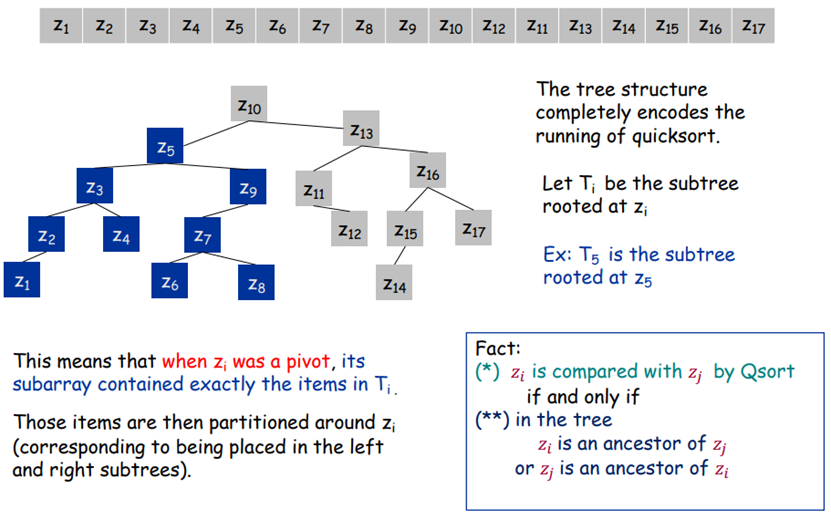
\includegraphics[width=0.8\textwidth]{img4-1}
\end{figure}

\subsubsection{Expected Running Time for Random-Based Quicksort} 

$\bullet$ Two elements $z_i$ and $z_j$ are compared at most once, iff $z_i$ or $z_j$ is the first to be chosen among $z_i, \cdots, z_j$

$\bullet$ The probability above (any indicated two elements $z_i$ and $z_j$ are compared) is $\frac{2}{j-1+1}$

$$
\implies E_{\text{Num of comparisons made}} = \sum_{i<j} \frac{2}{j-1+1} = O(n\log n)
$$

\subsubsection{Find the i-th Smallest Element Using Quicksort}

\begin{formal}{Brown}{brownshade}
	
	\textbf{Example: Find the i-th Smallest Element}
	
	Given an unsorted array $A[1\dots n]$ and an integer $i$, return the $i$-th smallest element of $A[1\dots n]$.
	
\vspace*{1em}

\noindent \textbf{Idea:}

\noindent 1. Choose a Pivot $x$ from $A[p\dots r]$

\noindent 2. Partition $A$ around $x$. (linear time)

\noindent 3. After partitioning, pivot $x$ will be at known location $q$

If $i = q-p+1$, then $x$ is the actual solution

If $i < q-p+1$, then the $i$-th element of $A[p\dots r]$ is the $i$-th element of $A[p\dots q-1]$, solve recursively

If $i > q-p+1$, then the $i$-th element of $A[p\dots r]$ is the $j = (i-q+p-1)$-th element of $A[q+1\dots r]$, solve recursively

\end{formal}

\begin{algorithm}
	\SetAlgoLined
	\SetKwFunction{Select}{Select}
	\Select{$A, p, r, i$}{
		
		\If{$p=r$}{
			\Return{$A[p]$}
		}
		
		Randomly choose an element in $A[p\dots r]$ as the pivot and swap it with $A[r]$
		
		$q$ \gets Partition($A, p, r$)
		
		$k$ \gets $q-p+1$
		
		\If{$i=k$}{
			\Return{$A[q]$}
		}
	
		\ElseIf{$i<k$}{
			
			\Return{\Select{$A, p, q-1, i$}}
			
		}

		\Else{
		
			\Return{\Select{$A, q+1, r, i-k$}}
		
		}
		
	}
	
	\underline{First Call:} \Select{$A, 1, n, i$}
	
	\caption{i-th Smallest Element}
\end{algorithm}

\subsubsection{Expected Running Time for Finding the i-th Smallest Element}

$\bullet$ A pivot is "good" if it's between the 25\%- and 75\%-percentile of sorted $A$, eliminating at least 1/4 of the array. The probability for such "good" pivot is 1/2.

$\bullet$ Let $i$-th stage be the time between the $i$-th good pivot (not including) and the $(i+1)$-st good pivot (including), $i=0, 1, 2, \cdots$, then the expected pivots selected within a stage is 2.

$\bullet$ Let $Y_i =$ the running time of $i$-th stage, $X_i =$ the num. of pivots (recursive calls) in $i$-th stage. Then $Y_i \leq X_i (3/4)^i n$.
$$
\implies E[Y_i] \leq E[X_i (3/4)^i n] = 2(3/4)^i n \implies \text{Expected Total Running Time} \leq E[\sum_i Y_i] \leq \sum_i 2(3/4)^i n = O(n)
$$

\begin{formal}{Brown}{brownshade}
	
	\textbf{Example: i-th Smallest Element in Two Sorted Arrays}
	
	Given two sorted arrays $A1$ and $A2$ of sizes $m$ and $n$. Design an
	algorithm to find the $k$-th smallest element in the union of the elements in $A1$ and $A2$ $(k \leq m+n)$.
	
\end{formal}

\begin{algorithm}
	\SetAlgoLined
	\SetKwFunction{Search}{Search}
	\Search{$\text{array }A1, \text{array }A2, \text{start1 }1, \text{end1 }k, \text{start2 }1, \text{end2 }k, \text{Order }k$}{
		
		\textbf{Main Idea:} Compare elements $A1[k/2]$ and $A2[k/2]$
		
		\If{$A1[k/2] < A2[k/2]$}{
			
			Eliminate first half of $A1$
			
			\Return{\Search{$A1, A2, k/2+1, \text{end1}, \text{start2}, \text{end2}, k/2$}}
			
		}
		
		\Else{
		
			Eliminate first half of $A2$
			
			\Return{\Search{$A1, A2, \text{start1}, \text{end1}, k/2+1, \text{end2}, k/2$}}
		
		}
		
	}
	
	\caption{i-th Smallest Element in Two Sorted Arrays}
\end{algorithm}

\textbf{Time Complexity:} $\Theta(\log k)$

\newpage

\subsection{Heapsort}

\subsubsection{Priority Queues}

\textbf{Main Idea:} Processing the shortest job first - Extracting the smallest element from the queue.

A Priority Queue is an abstract data structure that supports two 
operations: Insert \& Extract-Min.

\textbf{Implementations:}

1. Unsorted list + a pointer to the smallest element: $O(1)$ Insert \& $O(n)$ Extract-Min

2. Sorted doubly linked list + a pointer to first element: $O(n)$ Insert \& $O(1)$ Extract-Min

\subsubsection{Binary Heap Implementation}

$\bullet$ All levels are full except possibly the lowest level

$\bullet$ If the lowest level is not full, then nodes must be packed to 
the left

$\bullet$ The value of a node is at least the value of its parent — Min-heap

$\bullet$ Both Insert \& Extract-Min can be done in $O(\log n)$ time

\begin{formal}{DarkBlue}{blueshade}
	
	\textbf{Notice}
	
	The binary tree here is DIFFERENT from the Binary Search Tree, which requires ALL left nodes $<$ parent, while ALL right nodes $>$ parent.
	
\end{formal}

\textbf{Array Implementation of Heap}

$\bullet$ The root is in array position 1

$\bullet$ For any element in array position $i$, the left child is in position $2i$, the right child is in position $2i+1$, the parent is in position $\lfloor i/2 \rfloor$

\begin{figure}[h]
	\centering
	\begin{subfigure}[b]{0.2\textwidth}
		\centering
		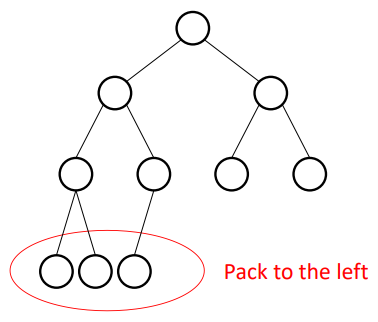
\includegraphics[width=\textwidth]{img4-2}
		%\caption{}
	\end{subfigure}
	%\hfill
	\begin{subfigure}[b]{0.5\textwidth}
		\centering
		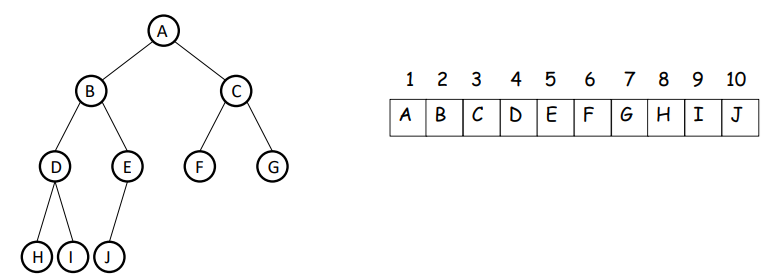
\includegraphics[width=\textwidth]{img4-3}
		%\caption{}
	\end{subfigure}
	%\caption{}
\end{figure}

\subsubsection{Heapsort}

\textbf{Insert}

$\bullet$ Add the new element to the next available position at the lowest level.

$\bullet$ Restore the min-heap property if violated.
\begin{algorithm}
	\SetAlgoLined
	\SetKwFunction{Insert}{Insert}
	\Insert{$x, i$}{
		
		$A[i]$ \gets $x$
		
		$j=i$
		
		\While(// $A[j]$ is less than its parent){$j>1$ and $A[j] < A[\lfloor j/2 \rfloor]$}{
			
			Swap $A[j]$ and $A[\lfloor j/2 \rfloor]$
			
		}
	
		$j=\lfloor j/2 \rfloor$
		
	}
	
	\caption{Add item $x$ to heap $A[1 \dots i-1]$}
\end{algorithm}

\textbf{Time Complexity:} $O(\log n)$

\newpage

\textbf{Extract-Min:} Should preserve both min-heap property \& completeness

$\bullet$ Copy the last element to the root (overwrite).

$\bullet$ Restore the min-heap property by percolating (or bubbling 
down): if the element is larger than either of its children, then
interchange it with the smaller of its children.
\begin{algorithm}
	\SetAlgoLined
	\SetKwFunction{Extract}{Extract-Min}
	\Extract{$i$}{
		
		Output($A[1]$)
		
		Swap $A[1]$ and $A[i]$
		
		$A[i] = \infty$, $j = 1$, $l = A[2j]$, $r = A[2j+1]$ // Left \& Right Children
		
		\While( // if $A[j]$ is larger than a child, swap with the smaller child){$A[j] > \min(l, r)$}{
		
			\If{$l<r$}{
			
				Swap $A[j]$ with $A[2j]$, $j=2j$
			
			}
		
			\Else{
			
				Swap $A[j]$ with $A[2j+1]$, $j=2j+1$
			
			}

			$l=A[2j], r=A[2j+1]$

		}
		
	}
	
	\caption{Remove the smallest item $A[1]$ in the heap $A[1 \dots i]$}
\end{algorithm}

\textbf{Time Complexity:} $O(\log n)$

\textbf{Total Time Complexity:} Build a binary heap of $n$ elements \& Perform $n$ Extract-Min operations: $O(n\log n)$

\begin{formal}{Brown}{brownshade}
	
	\textbf{Example: Merging $k$ Sorted Arrays}
	
	Suppose that you have $k$ sorted arrays, each with $n$ elements, and you want to combine them into a single sorted array of $kn$ elements.

\textbf{Solution 1:} Merge the first two arrays, then merge it with the third, and so on. Time Complexity = $\sum_{i=2}^k in = O(k^2 n)$

\textbf{Solution 2:} Divide recursively $k$ sorted arrays into two parts, conduct the merging for the subproblems. $T(k) = 2T(k/2) + kn \implies \text{Time Complexity = }T(k) = O(kn\log k)$

\textbf{Solution 3 (Heapsort):} Insert the first element of each array into an empty min-heap. Extract-min every time and insert the next item of in the same array as the one being extracted. Time Complexity = $O(kn\log k)$

\end{formal}

\begin{formal}{Brown}{brownshade}

	\textbf{[Operation Implementation]}
	
	\textbf{Decrease-Key:} Decreases the value of one specified element (Used in Dijkstra's Algorithm)
	
	\textbf{Modification of the heaps to support it in $O(\log n)$ time:} Change the heap tree to a binary search tree.

\end{formal}

For more information, see: \href{https://en.wikipedia.org/wiki/Binary_heap}{Binary Heap (Wikipedia)}

Some websites markdown:
\href{https://www.zhihu.com/question/31387715}{Zhihu}
\href{http://www.matrix67.com/blog/archives/1209}{Web 1}
\href{http://www.matrix67.com/blog/archives/1523}{Web 2}


\newpage

\subsection{Linear-Time Sorting}

\subsubsection{Decision Trees and Lower Bounds}

\textbf{Decision Tree Model}
\begin{figure}[h]
	\centering
	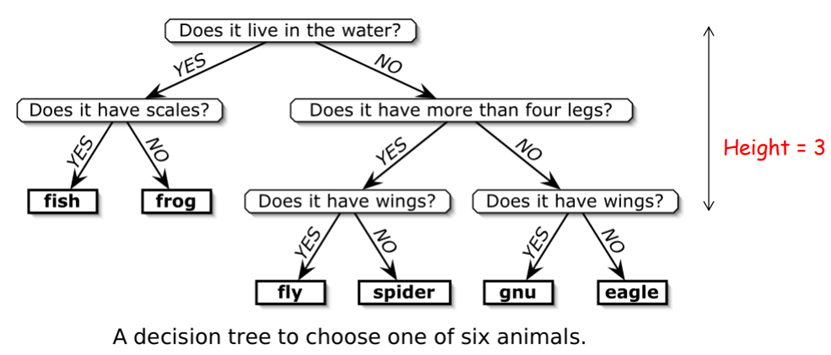
\includegraphics[width=0.6\textwidth]{img4-4}
\end{figure}

\textbf{Fact:} A binary tree with $n$ leaves must have height $\Omega(\log n)$.

\textbf{Theorem:} Any algorithm for finding location of given element in a sorted array of size $n$ must have running time $\Omega(\log n)$ in the decision-tree model.

\begin{formal}{Green}{greenshade}
	
	\textbf{Theorem:} Any \textbf{comparison-based sorting algorithm} (only by using comparisons without using thetr accurate values) requires $\Omega(n\log n)$ time.
	
	Given $n$ numbers, there are $n!$ possible permutations, resulting in the tree height being $\Omega(\log(n!))$. Thus, the time complexity is bounded as $\Omega(\log(n!)) = \Omega(n\log n)$.
	
\end{formal}

\subsubsection{Linear-time Sorting}

\textbf{Counting-Sort}

$\bullet$ Assumes that the elements are integers from 1 to $k$

\begin{algorithm}
	\SetAlgoLined
	\KwIn{$A[1\cdots n]$ where $A[j]\in {1,2,\cdots,k}$}
	\KwOut{$B[1\cdots n]$, sorted}
	\SetKwFunction{CountingSort}{Counting-Sort}
	
	\CountingSort{$A, B, k$}{
	
	Let $C[1\cdots k]$ be a new array
	
	\For( // Initialize Counters){$i \gets 1$ to $k$}{$C[i] \gets 0$}
	
	\For( // Count the number of each element){$j \gets 1$ to $n$}{$C[A[j]] \gets C[A[j]] + 1$}
	
	\For( // Count the accumulative number of elements){$i \gets 2$ to $k$}{$C[i] \gets C[i] + C[i-1]$}
	
	\For( // Move the items into proper location){$j \gets n$ to 1}{
	
		$B[C[A[j]]] \gets A[j]$
		
		$C[A[j]] \gets C[A[j]] - 1$
	
		}
	
	}
	
	\caption{Counting-Sort Algorithm}
\end{algorithm}

\textbf{Time Complexity:} $\Theta(n+k)$

\textbf{Space Complexity:} $\Theta(n+k)$

\newpage

\textbf{Radix-Sort}

\begin{algorithm}
	\SetAlgoLined
	\KwIn{An array of $n$ numbers, each has at most $d$ digits}
	\KwOut{A sorted array}
	\SetKwFunction{RadixSort}{Radix-Sort}
	\RadixSort{$A, d$}{
	
	\For{$i \gets 1$ to $d$}{
	
		Use Counting-Sort to sort array $A$ on digit $i$
	
		}
		
	}
	
	\caption{Radix-Sort Algorithm}
\end{algorithm}

\textbf{Time Complexity:} $\Theta(d(n+k))$

\subsection{Sorting Reprise \& Comparison}

\begin{center}
\renewcommand{\arraystretch}{1.5}
\begin{tabular}{|c|c|c|c|c|c|}
	\hline
	& Insertion Sort & Merge Sort & Quick Sort & Heap Sort & Radix Sort \\
	\hline
	Running Time & $\Theta(n^2)$ & $\Theta(n\log n)$ & $\Theta(n\log n)$ & $\Theta(n\log n)$ & $\Theta(d(n+k))$ \\
	\hline
	Randomized & No & No & Yes & No & No \\
	\hline
	Working Space & $\Theta(1)$ & $\Theta(n)$ & $\Theta(\log n)$ & $\Theta(1)$ & $\Theta(n+k)$ \\
	\hline
	Comparison-Based & Yes & Yes & Yes & Yes & No \\
	\hline
	Stable & Yes & Yes & No & No & Yes \\
	\hline
	Cache Performance & Good & Good & Good & Bad & Bad \\
	\hline
	Parallelization & No & Excellent & Good & No & No \\
	\hline
\end{tabular}
\end{center}




































\end{document}

\newpage

\section{Graph Algorithms}

\subsection{Breadth \& Depth First Search}

\subsection{Shortest Paths}

\subsection{Shortest Paths}

\subsection{Maximum Flow and Bipartite Matchings}

\section{AVL Trees}

\section{Basic String Matching}

\section{Hashing}








\newpage

\end{document}

\begin{comment}

\section*{Homework 1}

\textbf{Name: LIN, Xuanyu, SID: 20838295, Email Address: xlinbf@connect.ust.hk}

\begin{Problem}
	
	For each pair of expressions $(A, B)$ below, indicate whether $A$
	is $O, \Omega, \text{or } \Theta$ of B. List all applicable relations. No explanation is needed.
	
	\noindent (a) $A = n^3-100n$, $B = n^2+50n$
	
	\noindent (b) $A = \log_2(n^2)$, $B = \log_{2.7}(n^4)$
	
	\noindent (c) $A = 10^{10000}$, $B = \frac{n}{10^{10000}}$
	
	\noindent (d) $A = 2^{n\log n}$, $B = n^{10}+8n^2$
	
	\noindent (e) $A = 2^n$, $B = 2^{n+\log n}$
	
	\noindent (f) $A = 3^{3n}$, $B = 3^{2n}$
	
	\noindent (g) $A = (\sqrt{2})^{\log n}$, $B = \sqrt{\log n}$
	
\end{Problem}

\textbf{Solution.}
	
	(a) $A = \Omega(B)$
	
	(b) $A = O(B), A = \Omega(B), A = \Theta(B)$
	
	(c) $A = O(B)$
	
	(d) $A = \Omega(B)$
	
	(e) $A = O(B)$
	
	(f) $A = \Omega(B)$
	
	(g) $A = \Omega(B)$

\newpage

\begin{Problem}
	
	Derive asymptotic upper bounds for T(n) in the following recurrences. Make your bounds as tight as possible. You may assume that $n$ is a power of 2 for (a), $n$ is a power of 4 for (b), and $\sqrt{n}$ is always an integer for (c).
	
	\noindent (a) $T(1) = 1$; $T(n) = 4T(n/2) + n^2$ for $n>1$.
	
	\noindent (b) $T(1) = 1$; $T(n) = 16T(n/4) + n$ for $n>1$.
	
	\noindent (c) $T(2) = 1$; $T(n) = T(\sqrt{n}) + 1$ for $n>1$.
	
\end{Problem}

\textbf{Solution.}

(a)
$$
\begin{aligned}
	T(n) &= 4T(n/2) + n^2 = 4[4T(n/4) + (n/2)^2] + n^2 = 4\{4[4T(n/8) + (n/4)^2] + (n/2)^2\} + n^2\\
	&= 4\{4\{4\{\cdots [4T(1) + 2^2] + 4^2\} + \cdots + (n/4)^2\} + (n/2)^2\} + n^2\\
	&= 4^{\log_2 n} + 4^{\log_2 n - 1} \times 2^2 + 4^{\log_2 n - 2} \times 4^2 + \cdots + 4^{1} \times (n/2)^2 + n^2\\
	&= n^2 + \frac{n^2}{4} \times 2^2 + \frac{n^2}{4^2} \times 4^2 + \cdots + 4 \times (n/2)^2 + n^2\\
	&= n^2 (\log_2 n + 1) = O(n^2\log n)
\end{aligned}
$$

(b)
$$
\begin{aligned}
	T(n) &= 16T(n/4) + n = 16[16T(n/4^2) + n/4] + n = 16\{16[16T(n/4^3) + n/4^2] + n/4\} + n\\
	&= 16\{16\{16\{\cdots [16T(1) + 4] + 4^2\} + \cdots + n/4^2\} + n/4\} + n\\
	&= 16^{\log_4 n} + 16^{\log_4 n - 1} \times 4 + 16^{\log_4 n - 2} \times 4^2 + \cdots + 16^{1} \times n/4 + n\\
	&= n^2 + \frac{n^2}{4} + \frac{n^2}{4^2} + \cdots + 4n + n\\
	&= \frac{n-4n^2}{1-4} = \frac{4}{3} n^2 -\frac{1}{3} n = O(n^2)
\end{aligned}
$$

(c)
$$
\begin{aligned}
	T(n) &= T(\sqrt{n}) + 1 = T(n^{1/2^2}) + 2 = T(n^{1/2^3}) + 3 = \cdots = T(2) + \log_2 (\log_2 n) = O(\log_2 (\log_2 n))
\end{aligned}
$$

\newpage

\begin{Problem}
	
	\noindent (a) Describe a recursive algorithm that returns a list of all possible $n\times n$ binary arrays where $n$ is a positive input integer. An array is binary if each of its entry is either 0 or 1. You can either describe your algorithm in text or in a documented pseudocode. Make sure that your algorithm is recursive. Make sure that your description is understandable.
	
	\noindent (b) Write down the recurrence for the running time of your
	recursive algorithm in (a) with the boundary condition(s). Explain your notations. Solve your recurrence from scratch to obtain the
	the running time of your algorithm.
	
\end{Problem}

\textbf{Solution.}

(a) Main Idea: Recursively solve the problem by reducing the $k\times k$ array to $(k-1)\times (k-1)$ array. Then generate all the binary array of the remaining $1\times (k-1)$, $(k-1)\times 1$ and $1\times 1$ array. For each kind of array for the $(k-1)\times (k-1)$ array, we insert the remaining $(2k-1)$ elements into it, forming the $(k\times k)$ array.

\begin{algorithm}
	\SetAlgoLined
	\SetKwFunction{AllBinaryArrays}{AllBinaryArrays}
	\SetKwFunction{GenerateRemaining}{GenerateRemaining}
	\AllBinaryArrays{$n$}{
		
		EmptyArray $\gets$ array$[n][n]$
		
		ArrayList<Type=array$[n][n]$> $\gets [\ ]$
		
		\If{n = 1}{
		
			ArrayList.append(array$[n][n] = 0$, array$[n][n] = 1$) // Set the last element to 0 \& 1, others remaining 0
			
			\Return{ArrayList}
		
		}
		
		ArrayList\_1, ArrayList\_2, ArrayList\_3 $\gets$ \GenerateRemaining{$n$}
		
		PreviousArrayList$[\ ][2:n][2:n] \gets$ \AllBinaryArrays{$n-1$}
		
		// Insert the remaining $(2n-1)$ elements into the $n\times n$ array, forming all kinds of $(n\times n)$ array
		
		\ForEach{Combination of ArrayList\_1, ArrayList\_2, ArrayList\_3}{
		
			ArrayList.append(PreviousArrayList$[\ ][2:n][2:n]$.set(PreviousArrayList$[\ ][1][2:n]\gets$ ArrayList\_1, PreviousArrayList$[\ ][2:n][1]\gets$ ArrayList\_2, PreviousArrayList$[\ ][1][1]\gets$ ArrayList\_3))

		}
		
		\Return{ArrayList}
		
	}

	\vspace*{1em}
	
	/* Recursively generate all the kinds of $1\times (n-1)$, $(n-1)\times 1$ and $1\times 1$ array respectively */

	\GenerateRemaining{$n$}{
		
		ArrayList\_1<Type=array$[1][n-1]$> $\gets [\ ]$\\
		ArrayList\_2<Type=array$[n-1][1]$> $\gets [\ ]$\\
		ArrayList\_3<Type=array$[1][1]$> $\gets [\ ]$
		
		\If{$n=2$}{
		
			\Return{$[[0], [1]], [[0], [1]], [[0], [1]]$} // To be assigned to $1\times (n-1)$, $(n-1)\times 1$ and $1\times 1$ array

		}
		
		ArrayList\_1$[\ ][1][2:n-1]$, ArrayList\_2$[\ ][2:n-1][1]$, ArrayList\_3$[\ ][1][1]$ $\gets$ \GenerateRemaining{$n-1$} // Assign all possible cases of the previous arrays into all the array in the corresponing list
		
		// Set the new element inserted to be 0 and 1
		
		ArrayList\_1 = ArrayList\_1$[\ ][1][2:n-1]$.set$[\ ][1][1]\gets 0$ + ArrayList\_1$[\ ][1][2:n-1]$.set$[\ ][1][1]\gets 1$
		
		ArrayList\_2 = ArrayList\_2$[\ ][2:n-1][1]$.set$[\ ][1][1]\gets 0$ + ArrayList\_1$[\ ][2:n-1][1]$.set$[\ ][1][1]\gets 1$
		
		\Return{ArrayList\_1, ArrayList\_2, ArrayList\_3}
		
	}

	\underline{First Call:} \AllBinaryArrays{$n$}

	\caption{All $n\times n$ Binary Arrays}
\end{algorithm}

(b) \textbf{Recurrence:} Suppose $T(n) = T(n-1) + O(f(n))$

$f(n)$ contains generating the remaining $1\times (n-1)$, $(n-1)\times 1$ and $1\times 1$ arrays as well as inserting such arrays into the original $n\times n$ array. The first part requires $O(n)$ time as a simple recursion while the second part requires $O(n\times 2^n)$ time, considering the insertion time.

Thus,

$$
T(n) = T(n-1) + O(n\times 2^n) = \sum_{k=1}^n k\times 2^k = O(n2^n)
$$



\newpage

\begin{Problem}
	
	Let $A[1..n]$ be an array of $n$ elements. One can compare in $O(1)$ time two elements of $A$ to see if they are equal or not; however,
	the order relations $<$ and $>$ do not make sense. That is, one can check whether $A[i] = A[j]$ in $O(1)$ time, but the relations $A[i] < A[j]$ and $A[i] > A[j]$ are undefined and cannot be determined.
	
	\noindent In the tutorial you developed an $O(n\log n)$-time divide-and-conquer algorithm for finding a majority element of $A$ if one exists. In this assignment you need to generalize this problem.
	
	\noindent Let $k\in [1..n]$ be a fixed integer. An element of $A[1..n]$ is a k-major element if its number of occurrences in A is greater than $n/k$. For example, if $n = 30$, then a 10-major element should occur greater than 3 times (i.e., at least 4 times). Note that it is possible that no k-major exists for a particular k; it is also possible that there are multiple k-major elements for a particular k.
	
	\noindent This problem concerns with designing a divide-and-conquer algorithm for finding \textbf{all} 10-major elements in $A[1..n]$ in $O(n\log n)$ time; if there is no 10-major element, report so. Answer the following questions.
	
	(a) What is the maximum number of 10-major elements in
	$A[1..n]$? Explain.
	
	(b) Design a divide-and-conquer algorithm that finds all 10-major elements in $A[1..n]$ in $O(n\log n)$ time; if there is no 10-major element, your algorithm should report so. Recall that one can check whether $A[i] = A[j]$ in $O(1)$ time, but the relations $A[i] < A[j]$ and $A[i] > A[j]$ are undefined and cannot be computed.
	
	\noindent \textbf{Write your algorithm in documented pseudocode. Also, explain in text what your pseudocode does. Explain the correctness of your algorithm.}
	
	\noindent Since your algorithm uses the divide-and-conquer principle, it should
	be recursive in nature. That is, it should work on $A[1..n]$ in the
	first call to return all 10-major elements of $A[1..n]$, and in subsequent recursive calls, it may recurse on many subarrays $A[p..q]$ for some $p, q\in [1..n]$ to return all 10-major elements of $A[p..q]$
	
	\noindent Given a particular subarray $A[p..q]$, a 10-major element of $A[p..q]$ is not necessarily a 10-major element of $A[1..n]$. Conversely, a 10-major element of $A[1..n]$ is not necessarily a 10-major element of $A[p..q]$.
	
	(c) Derive a recurrence relation that describes the running time $T(n)$ of your algorithm. Explain your reasoning. State the boundary condition(s).
	
	(d) Solve your recurrence \textbf{from scratch} to show that $T(n) = O(n\log n)$.
	
\end{Problem}

\newpage

\textbf{Solution.}

(a) The maximum number of 10-major elements is 9. If there were 10 10-major elements in an array of $n$ numbers, each 10-major elements should appear at least $\lfloor n/10 \rfloor + 1$ times, resulting in a total of at least $10 \lfloor n/10 \rfloor + 10 > 10(n/10-1) + 10 = n$ numbers to be presented. For 9 10-major elements, supposing there are 100 numbers in total, each such elements appear 11 times would satisfy the requirement.

(b) Since the 10-major elements require the elements to appear at least $\lfloor n/10 \rfloor + 1$ times, we can infer that, if we cut the array into 10 subarrays, such elements must also be a 10-major elements in at least one of the subarray. Reporting such elements in the subarray to the previous recurrsion and checking if they are still 10-major elements in the previous recurrsion can help us get all the 10-major elements.

\begin{algorithm}
	\SetAlgoLined
	\SetKwFunction{GetMajorElements}{GetMajorElements}
	\GetMajorElements{$A[n]$}{
		
		\If{len($A$) = 0 or 1}{\Return{$A$}} // Return $A$ itself as it stores nothing or the only 10-major element
		
		PossibleMajorElements $\gets [\ ]$
		
		TrueMajorElements $\gets [\ ]$
		
		\For{$i \gets$ 0 to 9}{
			
			start $\gets \lceil ni/10 \rceil$
			
			end $\gets \lceil n(i+1)/10 \rceil - 1$
		
			PossibleMajorElements.append(\GetMajorElements{$A[start:end]$})

			// Check whether the elements in the PossibleMajorElements array are still 10-major elements in $A$
			
			\ForEach{elements in PossibleMajorElements}{
			
				Count its appearances in $A$, append it into TrueMajorElements if its appearances $\geq \lfloor n/10 \rfloor + 1$
		
			}

		}
		
		\Return{TrueMajorElements}
		
	}
	
	\underline{First Call:} \GetMajorElements{$A[n]$}
	
	\caption{Get All 10-Major Elements}
\end{algorithm}

Correctness: As any 10-major element must be a 10-major element in at least one of the subarray, we must get all the possible answers.

(c) \textbf{Recurrence:} Suppose $T(n) = 10T(n/10) + O(f(n))$ with $T(1) = 1$

$f(n)$ contains counting the appearance number of each element in PossibleMajorElements within the array $A$. We've derived that there are at most 9 10-major elements in any subarray, indicating that there are no more than $9\times 10 = 90$ candidates stored in PossibleMajorElements. Comparing such 90 elements to the original array $A$ costs $O(n)$ time complexity. Thus, $f(n) = n$

$$
T(n) = 10T(n/10) + O(n) \text{ with } T(1) = 1
$$

(d)
$$
T(n) = 10T(n/10) + O(n) = 100T(n/100) + 11n = 1000T(n/1000) + 111n = \cdots = 10^{\log_{10}n} T(1) + 100 n\log_{10} n = O(n\log n)
$$

\newpage

\end{comment}

\section*{Homework 2}

\textbf{Name: LIN, Xuanyu, SID: 20838295, Email Address: xlinbf@connect.ust.hk}

\begin{figure}[h]
	\centering
	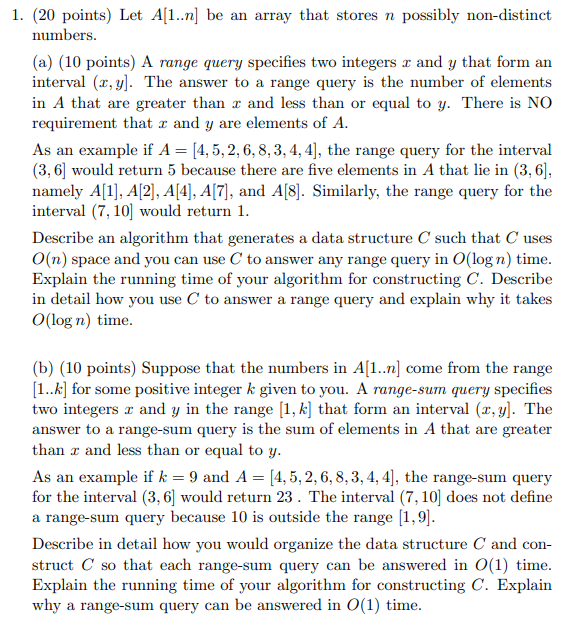
\includegraphics[width=0.6\textwidth]{hw2-1}
\end{figure}

\textbf{Solution.}

(a) Algorithm that generates the data structure $C$:
\begin{algorithm}
	\SetAlgoLined
	\SetKwFunction{Func}{Func}
	\Func{$A$}{
		
		\If{}{
			\Return
		}
		
		\For{}{
			
		}
		
		\Return{}
		
		\underline{First Call:} \Func{$$}
		
	}
	
	\caption{Func}
\end{algorithm}





\newpage

\begin{figure}[h]
	\centering
	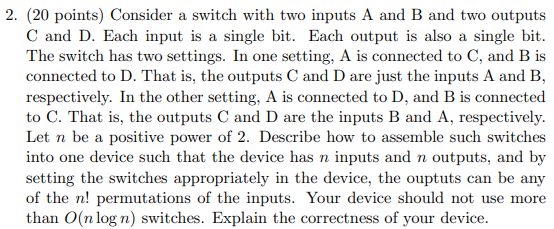
\includegraphics[width=0.6\textwidth]{hw2-2}
\end{figure}

\textbf{Solution.}

\newpage

\begin{figure}[h]
	\centering
	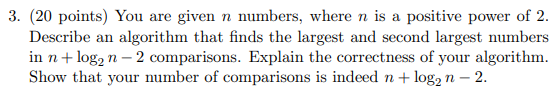
\includegraphics[width=0.6\textwidth]{hw2-3}
\end{figure}

\textbf{Solution.}

\begin{figure}[h]
	\centering
	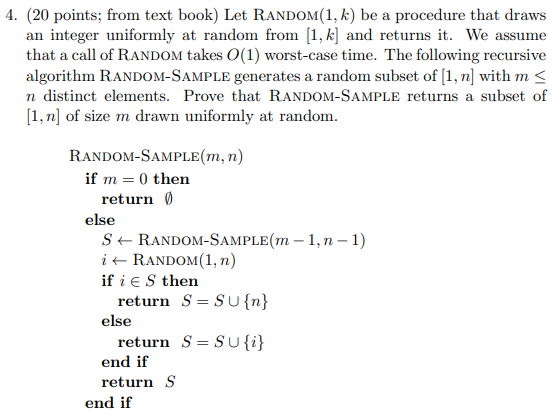
\includegraphics[width=0.6\textwidth]{hw2-4}
\end{figure}

\textbf{Solution.}

\newpage

\begin{figure}[h]
	\centering
	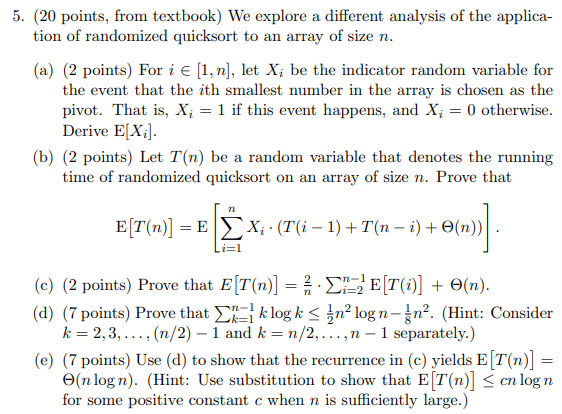
\includegraphics[width=0.6\textwidth]{hw2-5}
\end{figure}

\textbf{Solution.}

\newpage

\begin{Problem}
	
\end{Problem}

\textbf{Solution.}

\newpage

\begin{Problem}
	
\end{Problem}

\textbf{Solution.}

\newpage

\begin{Problem}
	
\end{Problem}

\textbf{Solution.}

\newpage

\begin{Problem}
	
\end{Problem}

\textbf{Solution.}

\newpage

\end{document}